\documentclass{article}
\usepackage{iclr2027_conference,times}
\usepackage{hyperref}
\usepackage{url}
\usepackage{booktabs}
\usepackage{graphicx}
\usepackage{amsmath}
\usepackage{amssymb}
%%%%% NEW MATH DEFINITIONS %%%%%

\usepackage{amsmath,amsfonts,bm}

% Mark sections of captions for referring to divisions of figures
\newcommand{\figleft}{{\em (Left)}}
\newcommand{\figcenter}{{\em (Center)}}
\newcommand{\figright}{{\em (Right)}}
\newcommand{\figtop}{{\em (Top)}}
\newcommand{\figbottom}{{\em (Bottom)}}
\newcommand{\captiona}{{\em (a)}}
\newcommand{\captionb}{{\em (b)}}
\newcommand{\captionc}{{\em (c)}}
\newcommand{\captiond}{{\em (d)}}

% Highlight a newly defined term
\newcommand{\newterm}[1]{{\bf #1}}


% Figure reference, lower-case.
\def\figref#1{figure~\ref{#1}}
% Figure reference, capital. For start of sentence
\def\Figref#1{Figure~\ref{#1}}
\def\twofigref#1#2{figures \ref{#1} and \ref{#2}}
\def\quadfigref#1#2#3#4{figures \ref{#1}, \ref{#2}, \ref{#3} and \ref{#4}}
% Section reference, lower-case.
\def\secref#1{section~\ref{#1}}
% Section reference, capital.
\def\Secref#1{Section~\ref{#1}}
% Reference to two sections.
\def\twosecrefs#1#2{sections \ref{#1} and \ref{#2}}
% Reference to three sections.
\def\secrefs#1#2#3{sections \ref{#1}, \ref{#2} and \ref{#3}}
% Reference to an equation, lower-case.
\def\eqref#1{equation~\ref{#1}}
% Reference to an equation, upper case
\def\Eqref#1{Equation~\ref{#1}}
% A raw reference to an equation---avoid using if possible
\def\plaineqref#1{\ref{#1}}
% Reference to a chapter, lower-case.
\def\chapref#1{chapter~\ref{#1}}
% Reference to an equation, upper case.
\def\Chapref#1{Chapter~\ref{#1}}
% Reference to a range of chapters
\def\rangechapref#1#2{chapters\ref{#1}--\ref{#2}}
% Reference to an algorithm, lower-case.
\def\algref#1{algorithm~\ref{#1}}
% Reference to an algorithm, upper case.
\def\Algref#1{Algorithm~\ref{#1}}
\def\twoalgref#1#2{algorithms \ref{#1} and \ref{#2}}
\def\Twoalgref#1#2{Algorithms \ref{#1} and \ref{#2}}
% Reference to a part, lower case
\def\partref#1{part~\ref{#1}}
% Reference to a part, upper case
\def\Partref#1{Part~\ref{#1}}
\def\twopartref#1#2{parts \ref{#1} and \ref{#2}}

\def\ceil#1{\lceil #1 \rceil}
\def\floor#1{\lfloor #1 \rfloor}
\def\1{\bm{1}}
\newcommand{\train}{\mathcal{D}}
\newcommand{\valid}{\mathcal{D_{\mathrm{valid}}}}
\newcommand{\test}{\mathcal{D_{\mathrm{test}}}}

\def\eps{{\epsilon}}


% Random variables
\def\reta{{\textnormal{$\eta$}}}
\def\ra{{\textnormal{a}}}
\def\rb{{\textnormal{b}}}
\def\rc{{\textnormal{c}}}
\def\rd{{\textnormal{d}}}
\def\re{{\textnormal{e}}}
\def\rf{{\textnormal{f}}}
\def\rg{{\textnormal{g}}}
\def\rh{{\textnormal{h}}}
\def\ri{{\textnormal{i}}}
\def\rj{{\textnormal{j}}}
\def\rk{{\textnormal{k}}}
\def\rl{{\textnormal{l}}}
% rm is already a command, just don't name any random variables m
\def\rn{{\textnormal{n}}}
\def\ro{{\textnormal{o}}}
\def\rp{{\textnormal{p}}}
\def\rq{{\textnormal{q}}}
\def\rr{{\textnormal{r}}}
\def\rs{{\textnormal{s}}}
\def\rt{{\textnormal{t}}}
\def\ru{{\textnormal{u}}}
\def\rv{{\textnormal{v}}}
\def\rw{{\textnormal{w}}}
\def\rx{{\textnormal{x}}}
\def\ry{{\textnormal{y}}}
\def\rz{{\textnormal{z}}}

% Random vectors
\def\rvepsilon{{\mathbf{\epsilon}}}
\def\rvtheta{{\mathbf{\theta}}}
\def\rva{{\mathbf{a}}}
\def\rvb{{\mathbf{b}}}
\def\rvc{{\mathbf{c}}}
\def\rvd{{\mathbf{d}}}
\def\rve{{\mathbf{e}}}
\def\rvf{{\mathbf{f}}}
\def\rvg{{\mathbf{g}}}
\def\rvh{{\mathbf{h}}}
\def\rvu{{\mathbf{i}}}
\def\rvj{{\mathbf{j}}}
\def\rvk{{\mathbf{k}}}
\def\rvl{{\mathbf{l}}}
\def\rvm{{\mathbf{m}}}
\def\rvn{{\mathbf{n}}}
\def\rvo{{\mathbf{o}}}
\def\rvp{{\mathbf{p}}}
\def\rvq{{\mathbf{q}}}
\def\rvr{{\mathbf{r}}}
\def\rvs{{\mathbf{s}}}
\def\rvt{{\mathbf{t}}}
\def\rvu{{\mathbf{u}}}
\def\rvv{{\mathbf{v}}}
\def\rvw{{\mathbf{w}}}
\def\rvx{{\mathbf{x}}}
\def\rvy{{\mathbf{y}}}
\def\rvz{{\mathbf{z}}}

% Elements of random vectors
\def\erva{{\textnormal{a}}}
\def\ervb{{\textnormal{b}}}
\def\ervc{{\textnormal{c}}}
\def\ervd{{\textnormal{d}}}
\def\erve{{\textnormal{e}}}
\def\ervf{{\textnormal{f}}}
\def\ervg{{\textnormal{g}}}
\def\ervh{{\textnormal{h}}}
\def\ervi{{\textnormal{i}}}
\def\ervj{{\textnormal{j}}}
\def\ervk{{\textnormal{k}}}
\def\ervl{{\textnormal{l}}}
\def\ervm{{\textnormal{m}}}
\def\ervn{{\textnormal{n}}}
\def\ervo{{\textnormal{o}}}
\def\ervp{{\textnormal{p}}}
\def\ervq{{\textnormal{q}}}
\def\ervr{{\textnormal{r}}}
\def\ervs{{\textnormal{s}}}
\def\ervt{{\textnormal{t}}}
\def\ervu{{\textnormal{u}}}
\def\ervv{{\textnormal{v}}}
\def\ervw{{\textnormal{w}}}
\def\ervx{{\textnormal{x}}}
\def\ervy{{\textnormal{y}}}
\def\ervz{{\textnormal{z}}}

% Random matrices
\def\rmA{{\mathbf{A}}}
\def\rmB{{\mathbf{B}}}
\def\rmC{{\mathbf{C}}}
\def\rmD{{\mathbf{D}}}
\def\rmE{{\mathbf{E}}}
\def\rmF{{\mathbf{F}}}
\def\rmG{{\mathbf{G}}}
\def\rmH{{\mathbf{H}}}
\def\rmI{{\mathbf{I}}}
\def\rmJ{{\mathbf{J}}}
\def\rmK{{\mathbf{K}}}
\def\rmL{{\mathbf{L}}}
\def\rmM{{\mathbf{M}}}
\def\rmN{{\mathbf{N}}}
\def\rmO{{\mathbf{O}}}
\def\rmP{{\mathbf{P}}}
\def\rmQ{{\mathbf{Q}}}
\def\rmR{{\mathbf{R}}}
\def\rmS{{\mathbf{S}}}
\def\rmT{{\mathbf{T}}}
\def\rmU{{\mathbf{U}}}
\def\rmV{{\mathbf{V}}}
\def\rmW{{\mathbf{W}}}
\def\rmX{{\mathbf{X}}}
\def\rmY{{\mathbf{Y}}}
\def\rmZ{{\mathbf{Z}}}

% Elements of random matrices
\def\ermA{{\textnormal{A}}}
\def\ermB{{\textnormal{B}}}
\def\ermC{{\textnormal{C}}}
\def\ermD{{\textnormal{D}}}
\def\ermE{{\textnormal{E}}}
\def\ermF{{\textnormal{F}}}
\def\ermG{{\textnormal{G}}}
\def\ermH{{\textnormal{H}}}
\def\ermI{{\textnormal{I}}}
\def\ermJ{{\textnormal{J}}}
\def\ermK{{\textnormal{K}}}
\def\ermL{{\textnormal{L}}}
\def\ermM{{\textnormal{M}}}
\def\ermN{{\textnormal{N}}}
\def\ermO{{\textnormal{O}}}
\def\ermP{{\textnormal{P}}}
\def\ermQ{{\textnormal{Q}}}
\def\ermR{{\textnormal{R}}}
\def\ermS{{\textnormal{S}}}
\def\ermT{{\textnormal{T}}}
\def\ermU{{\textnormal{U}}}
\def\ermV{{\textnormal{V}}}
\def\ermW{{\textnormal{W}}}
\def\ermX{{\textnormal{X}}}
\def\ermY{{\textnormal{Y}}}
\def\ermZ{{\textnormal{Z}}}

% Vectors
\def\vzero{{\bm{0}}}
\def\vone{{\bm{1}}}
\def\vmu{{\bm{\mu}}}
\def\vtheta{{\bm{\theta}}}
\def\va{{\bm{a}}}
\def\vb{{\bm{b}}}
\def\vc{{\bm{c}}}
\def\vd{{\bm{d}}}
\def\ve{{\bm{e}}}
\def\vf{{\bm{f}}}
\def\vg{{\bm{g}}}
\def\vh{{\bm{h}}}
\def\vi{{\bm{i}}}
\def\vj{{\bm{j}}}
\def\vk{{\bm{k}}}
\def\vl{{\bm{l}}}
\def\vm{{\bm{m}}}
\def\vn{{\bm{n}}}
\def\vo{{\bm{o}}}
\def\vp{{\bm{p}}}
\def\vq{{\bm{q}}}
\def\vr{{\bm{r}}}
\def\vs{{\bm{s}}}
\def\vt{{\bm{t}}}
\def\vu{{\bm{u}}}
\def\vv{{\bm{v}}}
\def\vw{{\bm{w}}}
\def\vx{{\bm{x}}}
\def\vy{{\bm{y}}}
\def\vz{{\bm{z}}}

% Elements of vectors
\def\evalpha{{\alpha}}
\def\evbeta{{\beta}}
\def\evepsilon{{\epsilon}}
\def\evlambda{{\lambda}}
\def\evomega{{\omega}}
\def\evmu{{\mu}}
\def\evpsi{{\psi}}
\def\evsigma{{\sigma}}
\def\evtheta{{\theta}}
\def\eva{{a}}
\def\evb{{b}}
\def\evc{{c}}
\def\evd{{d}}
\def\eve{{e}}
\def\evf{{f}}
\def\evg{{g}}
\def\evh{{h}}
\def\evi{{i}}
\def\evj{{j}}
\def\evk{{k}}
\def\evl{{l}}
\def\evm{{m}}
\def\evn{{n}}
\def\evo{{o}}
\def\evp{{p}}
\def\evq{{q}}
\def\evr{{r}}
\def\evs{{s}}
\def\evt{{t}}
\def\evu{{u}}
\def\evv{{v}}
\def\evw{{w}}
\def\evx{{x}}
\def\evy{{y}}
\def\evz{{z}}

% Matrix
\def\mA{{\bm{A}}}
\def\mB{{\bm{B}}}
\def\mC{{\bm{C}}}
\def\mD{{\bm{D}}}
\def\mE{{\bm{E}}}
\def\mF{{\bm{F}}}
\def\mG{{\bm{G}}}
\def\mH{{\bm{H}}}
\def\mI{{\bm{I}}}
\def\mJ{{\bm{J}}}
\def\mK{{\bm{K}}}
\def\mL{{\bm{L}}}
\def\mM{{\bm{M}}}
\def\mN{{\bm{N}}}
\def\mO{{\bm{O}}}
\def\mP{{\bm{P}}}
\def\mQ{{\bm{Q}}}
\def\mR{{\bm{R}}}
\def\mS{{\bm{S}}}
\def\mT{{\bm{T}}}
\def\mU{{\bm{U}}}
\def\mV{{\bm{V}}}
\def\mW{{\bm{W}}}
\def\mX{{\bm{X}}}
\def\mY{{\bm{Y}}}
\def\mZ{{\bm{Z}}}
\def\mBeta{{\bm{\beta}}}
\def\mPhi{{\bm{\Phi}}}
\def\mLambda{{\bm{\Lambda}}}
\def\mSigma{{\bm{\Sigma}}}

% Tensor
\DeclareMathAlphabet{\mathsfit}{\encodingdefault}{\sfdefault}{m}{sl}
\SetMathAlphabet{\mathsfit}{bold}{\encodingdefault}{\sfdefault}{bx}{n}
\newcommand{\tens}[1]{\bm{\mathsfit{#1}}}
\def\tA{{\tens{A}}}
\def\tB{{\tens{B}}}
\def\tC{{\tens{C}}}
\def\tD{{\tens{D}}}
\def\tE{{\tens{E}}}
\def\tF{{\tens{F}}}
\def\tG{{\tens{G}}}
\def\tH{{\tens{H}}}
\def\tI{{\tens{I}}}
\def\tJ{{\tens{J}}}
\def\tK{{\tens{K}}}
\def\tL{{\tens{L}}}
\def\tM{{\tens{M}}}
\def\tN{{\tens{N}}}
\def\tO{{\tens{O}}}
\def\tP{{\tens{P}}}
\def\tQ{{\tens{Q}}}
\def\tR{{\tens{R}}}
\def\tS{{\tens{S}}}
\def\tT{{\tens{T}}}
\def\tU{{\tens{U}}}
\def\tV{{\tens{V}}}
\def\tW{{\tens{W}}}
\def\tX{{\tens{X}}}
\def\tY{{\tens{Y}}}
\def\tZ{{\tens{Z}}}


% Graph
\def\gA{{\mathcal{A}}}
\def\gB{{\mathcal{B}}}
\def\gC{{\mathcal{C}}}
\def\gD{{\mathcal{D}}}
\def\gE{{\mathcal{E}}}
\def\gF{{\mathcal{F}}}
\def\gG{{\mathcal{G}}}
\def\gH{{\mathcal{H}}}
\def\gI{{\mathcal{I}}}
\def\gJ{{\mathcal{J}}}
\def\gK{{\mathcal{K}}}
\def\gL{{\mathcal{L}}}
\def\gM{{\mathcal{M}}}
\def\gN{{\mathcal{N}}}
\def\gO{{\mathcal{O}}}
\def\gP{{\mathcal{P}}}
\def\gQ{{\mathcal{Q}}}
\def\gR{{\mathcal{R}}}
\def\gS{{\mathcal{S}}}
\def\gT{{\mathcal{T}}}
\def\gU{{\mathcal{U}}}
\def\gV{{\mathcal{V}}}
\def\gW{{\mathcal{W}}}
\def\gX{{\mathcal{X}}}
\def\gY{{\mathcal{Y}}}
\def\gZ{{\mathcal{Z}}}

% Sets
\def\sA{{\mathbb{A}}}
\def\sB{{\mathbb{B}}}
\def\sC{{\mathbb{C}}}
\def\sD{{\mathbb{D}}}
% Don't use a set called E, because this would be the same as our symbol
% for expectation.
\def\sF{{\mathbb{F}}}
\def\sG{{\mathbb{G}}}
\def\sH{{\mathbb{H}}}
\def\sI{{\mathbb{I}}}
\def\sJ{{\mathbb{J}}}
\def\sK{{\mathbb{K}}}
\def\sL{{\mathbb{L}}}
\def\sM{{\mathbb{M}}}
\def\sN{{\mathbb{N}}}
\def\sO{{\mathbb{O}}}
\def\sP{{\mathbb{P}}}
\def\sQ{{\mathbb{Q}}}
\def\sR{{\mathbb{R}}}
\def\sS{{\mathbb{S}}}
\def\sT{{\mathbb{T}}}
\def\sU{{\mathbb{U}}}
\def\sV{{\mathbb{V}}}
\def\sW{{\mathbb{W}}}
\def\sX{{\mathbb{X}}}
\def\sY{{\mathbb{Y}}}
\def\sZ{{\mathbb{Z}}}

% Entries of a matrix
\def\emLambda{{\Lambda}}
\def\emA{{A}}
\def\emB{{B}}
\def\emC{{C}}
\def\emD{{D}}
\def\emE{{E}}
\def\emF{{F}}
\def\emG{{G}}
\def\emH{{H}}
\def\emI{{I}}
\def\emJ{{J}}
\def\emK{{K}}
\def\emL{{L}}
\def\emM{{M}}
\def\emN{{N}}
\def\emO{{O}}
\def\emP{{P}}
\def\emQ{{Q}}
\def\emR{{R}}
\def\emS{{S}}
\def\emT{{T}}
\def\emU{{U}}
\def\emV{{V}}
\def\emW{{W}}
\def\emX{{X}}
\def\emY{{Y}}
\def\emZ{{Z}}
\def\emSigma{{\Sigma}}

% entries of a tensor
% Same font as tensor, without \bm wrapper
\newcommand{\etens}[1]{\mathsfit{#1}}
\def\etLambda{{\etens{\Lambda}}}
\def\etA{{\etens{A}}}
\def\etB{{\etens{B}}}
\def\etC{{\etens{C}}}
\def\etD{{\etens{D}}}
\def\etE{{\etens{E}}}
\def\etF{{\etens{F}}}
\def\etG{{\etens{G}}}
\def\etH{{\etens{H}}}
\def\etI{{\etens{I}}}
\def\etJ{{\etens{J}}}
\def\etK{{\etens{K}}}
\def\etL{{\etens{L}}}
\def\etM{{\etens{M}}}
\def\etN{{\etens{N}}}
\def\etO{{\etens{O}}}
\def\etP{{\etens{P}}}
\def\etQ{{\etens{Q}}}
\def\etR{{\etens{R}}}
\def\etS{{\etens{S}}}
\def\etT{{\etens{T}}}
\def\etU{{\etens{U}}}
\def\etV{{\etens{V}}}
\def\etW{{\etens{W}}}
\def\etX{{\etens{X}}}
\def\etY{{\etens{Y}}}
\def\etZ{{\etens{Z}}}

% The true underlying data generating distribution
\newcommand{\pdata}{p_{\rm{data}}}
% The empirical distribution defined by the training set
\newcommand{\ptrain}{\hat{p}_{\rm{data}}}
\newcommand{\Ptrain}{\hat{P}_{\rm{data}}}
% The model distribution
\newcommand{\pmodel}{p_{\rm{model}}}
\newcommand{\Pmodel}{P_{\rm{model}}}
\newcommand{\ptildemodel}{\tilde{p}_{\rm{model}}}
% Stochastic autoencoder distributions
\newcommand{\pencode}{p_{\rm{encoder}}}
\newcommand{\pdecode}{p_{\rm{decoder}}}
\newcommand{\precons}{p_{\rm{reconstruct}}}

\newcommand{\laplace}{\mathrm{Laplace}} % Laplace distribution

\newcommand{\E}{\mathbb{E}}
\newcommand{\Ls}{\mathcal{L}}
\newcommand{\R}{\mathbb{R}}
\newcommand{\emp}{\tilde{p}}
\newcommand{\lr}{\alpha}
\newcommand{\reg}{\lambda}
\newcommand{\rect}{\mathrm{rectifier}}
\newcommand{\softmax}{\mathrm{softmax}}
\newcommand{\sigmoid}{\sigma}
\newcommand{\softplus}{\zeta}
\newcommand{\KL}{D_{\mathrm{KL}}}
\newcommand{\Var}{\mathrm{Var}}
\newcommand{\standarderror}{\mathrm{SE}}
\newcommand{\Cov}{\mathrm{Cov}}
% Wolfram Mathworld says $L^2$ is for function spaces and $\ell^2$ is for vectors
% But then they seem to use $L^2$ for vectors throughout the site, and so does
% wikipedia.
\newcommand{\normlzero}{L^0}
\newcommand{\normlone}{L^1}
\newcommand{\normltwo}{L^2}
\newcommand{\normlp}{L^p}
\newcommand{\normmax}{L^\infty}

\newcommand{\parents}{Pa} % See usage in notation.tex. Chosen to match Daphne's book.

\DeclareMathOperator*{\argmax}{arg\,max}
\DeclareMathOperator*{\argmin}{arg\,min}

\DeclareMathOperator{\sign}{sign}
\DeclareMathOperator{\Tr}{Tr}
\let\ab\allowbreak

\hypersetup{pdftitle={Does Similarity-Based Stopping Make Retrieval More Effective?},pdfauthor={},pdfsubject={Anonymous coursework report draft}}
\title{Does Similarity-Based Stopping\\Make Retrieval More Effective?}
\author{Anonymous coursework submission}
\begin{document}
\maketitle
\lhead{Under review as a report for UoE 26/27 Sem1 INFR11269: Machine Learning Systems}

\section{Research question and system}
Fixed top-$k$ retrieval gives every query the same number of documents, regardless of the similarity scores. A cutoff can instead return a short prefix for an apparently specific query and a longer one when many documents have similar scores. This seems a natural way to remove unnecessary evidence, but ``more effective'' can mean higher precision, greater coverage, fewer input tokens or better generated answers. These objectives need not agree.

Our question is: \emph{at matched labelled-evidence recall, do absolute similarity and top-score-relative gap cutoffs improve precision or token efficiency over fixed top-$k$, and do those retrieval differences improve downstream answer quality, cost or latency?} We compare three policy families. Retrieval curves sweep their parameters; final answer evaluation compares fixed top-5, top-10 and top-20 with the two dev-selected cutoffs.

The retrieval results support a conditional conclusion: cutoffs improve \emph{macro precision} at matched recall, while using more evidence tokens. Pooled precision does not show the same benefit. A separate final LLM evaluation measures whether the document-level differences translate into answer quality, cost and latency; a favourable retrieval metric alone cannot establish system improvement.

\subsection{Pipeline and implementation}
The supplied speech-driven RAG pipeline uses GLM-ASR-Nano to transcribe audio, \texttt{enc\_a} to embed the transcript, exact cosine search over 24,000 corpus records and an LLM to answer from the selected text. We retain the supplied model, encoder, corpus, interfaces, CPU references and answer rubric. Our additions are the required CUDA computations, controlled retrieval policies, parallel experiment/accounting scripts and saved-data analyses.

We implement RoPE with paired in-place rotations; RMSNorm/softmax with warp/block reductions and stable normalization; tiled GEMM with fused bias/GELU; and streaming grouped-query attention without a full score matrix. Publication/reuse barriers and tile padding are retained. The approach uses online normalization and IO-aware computation principles \citep{milakov2018,dao2022}, without substituting external libraries for the coursework kernels. All 33 official cases pass. Section~\ref{sec:asr} gives the integrated ablation; detailed mechanisms and checks are in Appendix~\ref{app:kernels}.

\subsection{Three retrieval rules without a candidate cap}
Let $s_{q1}\geq\cdots\geq s_{qM}$ be the common cosine ranking for query $q$, with $M=24{,}000$. Fixed top-$k$ returns the first $k$ records. Absolute selection returns scores $s_{qi}\geq\tau$; relative selection returns $s_{q1}-s_{qi}\leq\delta$. Relative means a score \emph{difference}, not a ratio. An empty cutoff returns top-1. Ties follow corpus row order.

Both cutoffs select a \emph{prefix} of the embedding ranking: a subset of a sufficiently large top-$K$ pool, not an arbitrary noncontiguous subset. We rank the entire corpus, so neither rule has an artificial document-count cap. This avoids confounding cutoff behaviour with the earlier top-20/top-50 ceilings. Lowering a threshold may produce a very large context; only the frozen operating points undergo generation, after an explicit context-size check.

\clearpage
\section{Experimental design and measurements}
\subsection{Data, tuning and separation of stages}
The course provides 350 practice and 125 dev query recordings, 24,000 corpus records and public relevance judgements (qrels), with no official test partition. An earlier study excluded 26 previously used practice queries and locked the remaining 324. This follow-up reuses those 324 evaluation queries after inspecting earlier results. It is therefore \emph{not a fresh confirmatory holdout}, although new tuning uses only the 125 dev queries.

Cutoffs maximise dev \emph{macro retrieval F1}, with ties preferring fewer mean documents. Absolute similarity uses 97 predeclared values from 0.75 to 0.99; relative gap uses 81 values from 0 to 0.08. The frozen values are \textbf{$\tau=0.8925$, $\delta=0.009$}, with dev F1 .2659/.2949. Fixed \textbf{$k=5,10,20$} are predeclared answer-evaluation controls, not selected from answer scores.

We reuse cached ASR transcripts and query vectors, then recompute a full exact cosine ranking on CPU. Stable sorting changes two earlier top-20 orderings; every method shares the new ranking. The frozen absolute/relative selections have maxima of 32/18 documents, respectively. Neither reaches 50 even though both can exceed it. All selected prompts fit without truncation; the largest across the five settings is 8,977 input tokens under the pinned tokenizer and prompt format.

The generator is Mistral Small 4 through OpenRouter (\texttt{mistralai/mistral-small-2603}); the final judge is Gemini 2.5 Flash. This matches a named course generator option, not ELM's serving implementation. Generation uses temperature 0.1 and a 2,048-token output cap; judging uses temperature zero and a 768-token cap. Reasoning is requested disabled. Twelve workers execute shuffled query/policy tasks with identical prompts and settings. Identical contexts still receive independent fresh generation.

All \textbf{1,620 answers} ($324\times5$) are saved before judging begins. Every row receives fresh generation in this same randomized batch. The judge sees the transcript, candidate answer and qrels-derived gold documents, but not the policy, selected IDs, similarities or parameters. A second shuffled pass judges every saved answer. There are no policy changes after judging. Request, response, token, cost and completion records are retained.

\subsection{Quality and cost definitions}
For selected set $S_q$, relevant set $G_q$ and hits $h_q=|S_q\cap G_q|$,
\begin{equation}
 \bar R=\frac1N\sum_q\frac{h_q}{|G_q|},\qquad
 \bar P=\frac1N\sum_q\frac{h_q}{|S_q|},\qquad
 P_{\rm micro}=\frac{\sum_q h_q}{\sum_q |S_q|}.
\end{equation}
Macro averages give each query equal weight; micro precision weights retrieved records. Unjudged records count as non-relevant. Neither metric establishes that all necessary answer facts are present: relevant records may repeat facts, and qrels may omit useful evidence \citep{joren2025}.

The frontier's additive cost is the sum of token counts of individual retrieved texts, using the pinned Mistral tokenizer. It excludes question/system text, labels and separators. The answer table instead reports \emph{actual full input tokens} from provider usage. These cost boundaries are intentionally labelled separately. Matched-recall fixed-$k$ baselines interpolate neighbouring settings, equivalent to query-independent random mixtures, not an oracle that chooses $k$ from relevance labels.

The supplied judge assigns correctness, grounding and completeness scores from 0--4; their sum divided by 12 is a rubric score, not accuracy. It can reward a qualified insufficient-evidence answer when gold evidence is inadequate. Paired query bootstraps use 5,000 resamples and recompute the matched-recall mixture. Intervals are exploratory, unadjusted for multiple comparisons and omit annotation/judge bias. API cost separates generation from evaluation. Downstream latency includes local selection/context construction and generation API service under concurrency; cached ASR, encoding and ranking are excluded.

\clearpage
\section{Retrieval results: precise per query, costly per token}
Figure~\ref{fig:retrieval} sweeps all three policy families over the full corpus; 3,103 plotted settings cover the full range. The displayed axes focus on practical budgets, not a hidden selection cap. Diamonds are the frozen dev settings. The appendix shows the full range through 100\% labelled recall.

\begin{figure}[h]
\centering
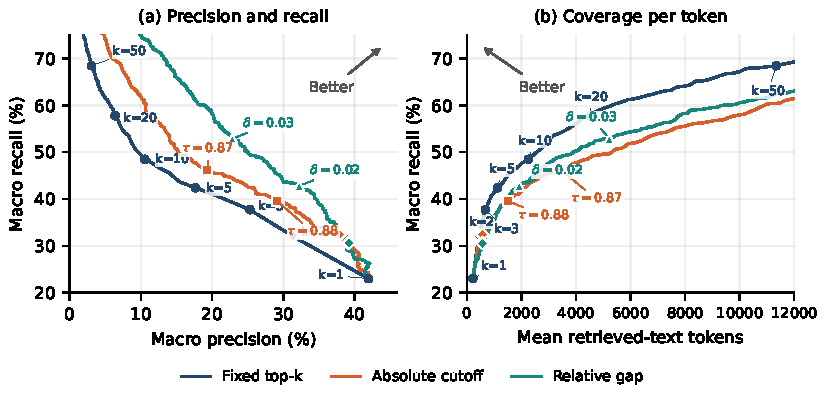
\includegraphics[width=\linewidth]{figures/uncapped-report-frontiers.pdf}
\caption{Uncapped selection on 324 queries. Cutoffs improve macro precision at similar recall but generally need more retrieved-text tokens in the displayed range. Diamonds denote dev-selected settings; curves are exploratory.}
\label{fig:retrieval}
\end{figure}

\begin{table}[h]
\centering
\caption{Frozen operating points; percentages are qrels metrics. Input tokens include the complete generation prompt. Bold marks highest quality or lowest token usage.}
\label{tab:retrieval}
\small
\begin{tabular}{lrrrrrr}
\toprule
Method & Mean docs & Max docs & Recall & Macro $P$ & Micro $P$ & Input tokens\\
\midrule
Fixed top-5 & 5.00 & 5 & 42.40 & 17.65 & 17.65 & 1227\\
Fixed top-10 & 10.00 & 10 & 48.46 & 10.56 & 10.56 & 2391\\
Fixed top-20 & 20.00 & 20 & \textbf{57.75} & 6.37 & 6.37 & 4730\\
Absolute cutoff & 2.40 & 32 & 32.39 & 37.89 & \textbf{28.41} & \textbf{657}\\
Relative gap & 2.55 & 18 & 30.60 & \textbf{39.21} & 23.34 & 667\\
\bottomrule
\end{tabular}
\end{table}

\textbf{Match recall before attributing a precision gain.} Absolute and relative achieve different recalls, so directly comparing their precision is incomplete. At absolute's 32.39\% recall, the fixed-$k$ mixture has 31.01\% macro precision versus 37.89\%; the gain is \textbf{6.87 percentage points}, with paired 95\% interval [3.02,10.97]. At relative's 30.60\% recall, its 39.21\% precision exceeds the mixture's 33.08\% by \textbf{6.13 points} [2.73,10.06].

\textbf{The gain costs more tokens at matched recall.} Absolute uses 566.6 retrieved-text tokens versus 456.5 for the fixed mixture, \textbf{24.1\% more}; relative uses 575.9 versus 407.3, \textbf{41.4\% more}. Additional-token intervals are [14.1,201.4] and [93.5,241.5]. Cutoffs use fewer tokens than the higher-recall fixed depths in Table~\ref{tab:retrieval}, but that does not demonstrate better token efficiency: the matched-recall comparison exposes the allocation penalty.

\textbf{Macro precision is not pooled efficiency.} Against the same matched-recall mixtures, absolute micro precision is 28.41\% versus 30.87\% (difference $-2.46$ points, interval [$-7.27,3.05$]); relative is 23.34\% versus 32.28\% ($-8.94$ points, [$-11.99,-5.48$]). The absolute pooled difference is uncertain, while relative's is clearly negative under this bootstrap. High macro precision can coexist with large low-precision selections on a smaller set of queries. Returning fewer records for many queries therefore need not reduce the total documents or tokens processed.

\clearpage
\section{Final answer evaluation and system cost}
Table~\ref{tab:answers} evaluates generated answers at the five predeclared settings, followed by separate policy-blind judging. Scores measure answer quality under the rubric; latency covers downstream service, not a new audio-to-answer benchmark.

\begin{table}[h]
\centering
\caption{Final evaluation, 324 queries per method. C/G/Comp are correctness/grounding/completeness, each out of 4. Score is their sum/12. Time is selection/context plus generation service under 12 workers. Dollars are generation per 1,000 queries, excluding judging. Bold marks best observed values, not significance.}
\label{tab:answers}
\small
\begin{tabular}{lrrrrrrr}
\toprule
Method & C & G & Comp & Score & Input & Time (s) & \$/1,000\\
\midrule
Fixed top-5 & 2.19 & 2.15 & 2.18 & 0.543 & 1227 & 2.75 & 0.363 \\
Fixed top-10 & 2.20 & 2.14 & 2.19 & 0.544 & 2391 & 3.08 & 0.581 \\
Fixed top-20 & 2.29 & 2.23 & 2.29 & 0.568 & 4730 & 3.50 & 0.987 \\
Absolute cutoff & \textbf{2.66} & \textbf{2.64} & \textbf{2.65} & \textbf{0.663} & \textbf{657} & \textbf{1.93} & \textbf{0.215} \\
Relative gap & 2.41 & 2.40 & 2.42 & 0.602 & 667 & 2.09 & 0.236 \\
\bottomrule
\end{tabular}
\end{table}

\textbf{Absolute cutoff scores higher than all three fixed depths.} Its mean score is .663, versus .543/.544/.568 for top-5/top-10/top-20. Paired gains are $+0.119$ [0.069,0.168], $+0.118$ [0.067,0.168] and $+0.095$ [0.045,0.143], respectively. It has the highest means in all three rubric dimensions and the lowest observed input tokens, latency and generation charge among the five rows. These comparisons are exploratory, with unadjusted intervals.

\textbf{Relative gap has a less consistent quality advantage.} Its .602 score exceeds top-5 by 0.058 [0.015,0.101] and top-10 by 0.057 [0.009,0.104]. Against top-20, the 0.034 difference has an interval spanning zero [$-0.011,0.078$]. Absolute exceeds relative by 0.061 [0.020,0.101]. Increasing fixed depth raises labelled recall substantially, but the judge-score means change much less.

\textbf{Shorter contexts reduce observed deployment costs here.} Relative to top-5, absolute cuts generation charges about 41\% and downstream latency by 0.816 s [$-0.949,-0.688$]; relative cuts charges about 35\% and latency by 0.658 s [$-0.777,-0.544$]. Against top-20, the time reductions are 1.569 and 1.411 s. Outputs average 232/260 tokens for the cutoffs versus 360/415/472 for top-5/top-10/top-20, so decoding length also changes. These settings are not recall-matched: lower absolute expenditure does not contradict worse token efficiency at a fixed recall.

All 1,620 answers finish below the output cap. Final judging yields 1,620 records from 1,627 calls. One explanation repeatedly contained unescaped quotation marks; all six attempts agreed on the numeric scores, which were retained unchanged in an explicitly logged JSON-format repair. All 3,247 charges reconcile: generation \$0.7719, judging \$1.0855, total \textbf{\$1.8573}. Earlier completed and interrupted runs are accounted for separately.


\subsection{What this comparison establishes}
The top-5/top-10/top-20 controls show what happens as the generator receives more retrieved evidence. Their recall and context sizes differ from the cutoffs, so answer-score gains alone cannot isolate adaptivity from using shorter contexts. The retrieval-only matched-recall analysis addresses allocation efficiency separately. The earlier top-2 comparison is retained as a diagnostic, not silently combined with this batch's latency or scores.

The judge dimensions are correlated, not independent replications. The rubric can favour qualified refusal and penalise valid information absent from qrels. Higher scores therefore need human-audited sufficiency/factuality checks before claiming better real-world task success.

Billing includes input and output; latency also depends on decoding, scheduling and concurrency. These associations do not isolate prefill cost. OpenRouter measurements do not establish ELM or local-GPU serving performance.

\clearpage
\section{Integrated ASR ablation and limitations}
\label{sec:asr}
Table~\ref{tab:asr} preserves ASR integration evidence; implementation details are in Appendix~\ref{app:kernels}. Measurements used an H200 MIG 1g.18gb slice (16 SMs), CUDA 12.8.93, PyTorch 2.10.0+cu128 and Transformers 5.0.0. The RAG ASR cache was produced separately on an RTX A6000; MIG times are not substituted into downstream latency.

\begin{table}[h]
\centering
\caption{ASR ablation on one 3.50-second recording. One warm-up and three timed runs per mode; loading excluded. All modes achieved 100\% supplied word accuracy on this clip. Memory is peak allocation.}
\label{tab:asr}
\begin{tabular}{lrr}
\toprule
Enabled custom groups & Time (ms) & Memory (GiB)\\
\midrule
None: framework reference & $1331.9\pm0.3$ & 8.90\\
RoPE + reductions & $1294.7\pm0.5$ & 8.90\\
Above + GEMM & $5144.9\pm0.1$ & 8.90\\
All four & $5672.1\pm0.4$ & 8.56\\
\bottomrule
\end{tabular}
\end{table}

All 33 official correctness cases and five additional shape/boundary cases pass. The all-CUDA model is nevertheless \textbf{4.26 times slower} than the framework reference, with peak allocated memory 0.34 GiB lower. In a separate instrumented profile, linear calls dominate (4,960.0 ms), followed by attention (688.6 ms). Less logical memory traffic does not reproduce optimized library register tiling and scheduling. The reductions-only improvement cannot compensate for slower GEMM. Mode order was fixed; the small run dispersion and one correctly transcribed clip do not establish general ASR speed or recognition accuracy.

\subsection{Threats to validity}
\textbf{Reused evaluation data.} The cleaner design was motivated by earlier observations on the same 324 queries. Dev-only tuning prevents direct test-threshold fitting, but cannot undo design-level test reuse. The curves, confidence intervals and final answer results are follow-up evidence. A new query set is needed for independent confirmation.

\textbf{Incomplete and redundant labels.} Qrels recall can require retrieving several interchangeable records, while precision can penalise unjudged useful evidence. Our primary claim is about these labelled-document metrics, not the minimum necessary context. Both macro and micro precision are required because they answer different questions. The previous stopped sufficiency/reranking studies are not silently completed or promoted into this comparison.

\textbf{One generator and judge.} Each query/policy has one answer and one valid judgement. Paired query intervals omit repeated-generation variability and judge bias. An earlier repeat-judge audit used other answers and does not validate this new evaluation.

\textbf{Measurement boundaries.} Exact retrieval is CPU-based on cached vectors; full-corpus sorting averaged about 2.09 ms in preparation. It is excluded from the downstream table, along with cached ASR/encoding and queue wait. The token frontier measures document-text volume, while billed prompt/output usage measures API expenditure. Neither is a direct GPU energy or isolated prefill-time measurement. Large-context sweep endpoints are retrieval analysis only, not demonstrated deployable generator configurations.

\section{Conclusion}
Uncapped cutoffs improve macro precision at matched recall but require more evidence tokens. Relative also loses pooled precision; absolute's pooled difference is uncertain. In final answer evaluation, absolute scores higher than top-5/top-10/top-20 while costing less; relative's score gain over top-20 is uncertain. These operating points have different recalls. Reporting both matched-recall efficiency and final-answer outcomes exposes the trade-off rather than declaring a universally better retriever.

\clearpage
\bibliography{references}
\bibliographystyle{iclr2027_conference}

\clearpage
\appendix
\section{CUDA implementation and detailed ablations}
\label{app:kernels}
\textbf{RoPE.} One thread owns a rotary dimension pair, reading both original values before writing. Q and K share a launch; indexing distinguishes head counts and resets positions per batch. Unrotated dimensions remain unchanged. Standard \texttt{sinf}/\texttt{cosf} preserve the supplied tolerance. Fast math failed the long-position case (maximum error $1.94\times10^{-4}$; 52,077 values outside tolerance), so it was rejected.

\textbf{Reductions.} Five XOR shuffle stages implement warp sums/maxima. Block reductions publish warp partials in shared memory with publication and reuse barriers. RMSNorm reduces squared values. Softmax combines stable summaries $(m,s)$ with $m=\max(m_a,m_b)$ and $s=s_a e^{m_a-m}+s_b e^{m_b-m}$; explicit empty identities avoid $-\infty-(-\infty)$. Two input passes replace the ordinary max/sum/write scheme's three \citep{milakov2018}. Removing the reuse barrier passed numerical tests but produced one racecheck error aggregating 160 hazards; the production barrier prevents scratch reuse before all readers finish \citep{nvidia2025}.

\textbf{GEMM.} Cooperative bounded loads feed shared input/transposed-weight tiles. Threads synchronize before tile consumption and reuse, including boundary threads. Bias and GELU are fused. Tile 16 remains the default because larger tiles trade dense-matrix efficiency against wasted rows in single-token projection. A $1024^3$ multiply reduces logical input requests 16-fold compared with naive scalar loads; fused encoder GELU avoids 61.44 MB of separate activation traffic. These are logical-byte estimates, not measured physical DRAM transfers.

\textbf{Attention.} Grouped query heads map to shared K/V heads. Streaming tiles update the running maximum, normalization sum and rescaled output accumulator, avoiding the full score matrix. This follows IO-aware principles \citep{dao2022}; the coursework implementation is not FlashAttention. Padding reduces shared-memory conflicts; four warps remain the validated default.

\begin{table}[h]
\centering
\caption{Selected kernel ablations on the same MIG allocation. Median over three timing rounds; the second reversed configuration order. Defaults are retained unless fully validated.}
\begin{tabular}{llr}
\toprule
Workload & Configuration & Time (ms)\\
\midrule
Encoder fc1 + GELU & Tile 16, padded / unpadded & 21.101 / 49.998\\
 & Tile 32, padded & 18.372\\
Vocabulary projection & Tile 16 / tile 32 & 4.060 / 7.138\\
Audio attention & Four warps, padded / unpadded K & 20.712 / 106.063\\
 & Eight warps, padded & 17.044\\
\bottomrule
\end{tabular}
\end{table}

All four RoPE, eleven reduction, ten GEMM and eight attention official cases pass, with unchanged references/tolerances. Five additional boundary/shape cases and reduction-helper checks pass. Largest default GEMM/attention errors are $3.72\times10^{-5}$/$5.21\times10^{-7}$. Small GEMM/attention and helper suites pass memcheck, racecheck and synccheck. Large cases receive numerical rather than exhaustive sanitizer coverage; the large-attention reference samples query rows. The tests establish correctness only for their covered cases.

\clearpage
\section{Full-range retrieval curves and evidence inventory}
\begin{figure}[h]
\centering
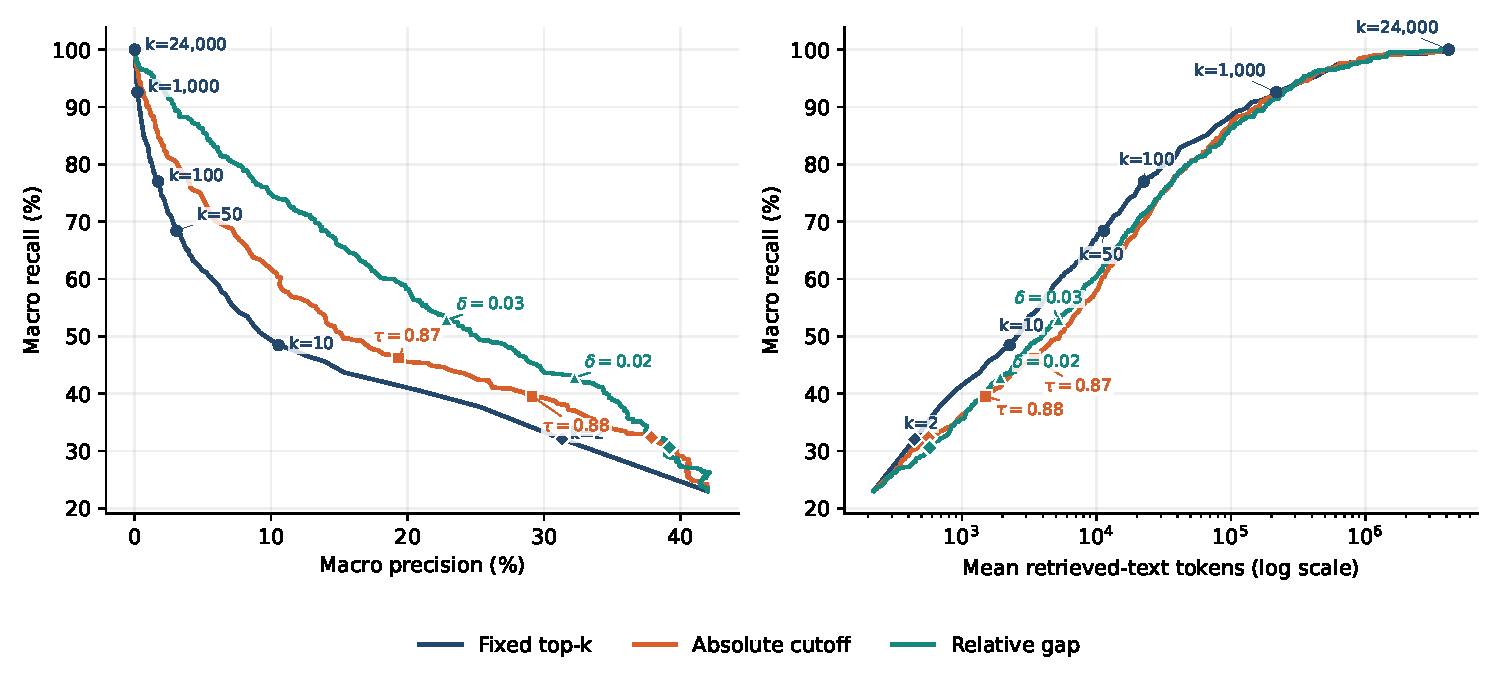
\includegraphics[width=\linewidth]{figures/uncapped-full-range.pdf}
\caption{Full-corpus sweeps extend to 100\% labelled recall. The log token axis exposes the cost of very low cutoffs. These endpoints were not passed to the generator; no artificial top-$K$ cap is hidden by the main figure's axis limits.}
\end{figure}

The final answer-evaluation run is \path{rag/results/cutoff-pipeline-20261116}. Its configuration, source hashes, frozen parameters, context preflight, 1,620 answers, raw judge responses, 1,620 final judgements, usage and reconciled billing records are retained. The generation-complete barrier precedes judge start. Dev tuning and retrieval frontiers are preserved in \path{rag/results/cutoff-uncapped-20261116}. The full-ranking cache contains 449 queries (125 dev plus 324 evaluation), each ranked against all 24,000 records. No new ASR, embedding-model or cross-encoder inference is needed.

Reproduction uses \path{rag/extensions/prepare_uncapped_rankings.py}, \path{rag/extensions/cutoff_pipeline_controls.py} and \path{rag/extensions/uncapped_frontiers.py}. The final compact plots/table come from \path{report/plot_uncapped_report.py}, with a separate \texttt{--evaluation-run} for the five-row answer table. The tokenizer is pinned to Mistral Small 4 revision \texttt{a11f36bebf709121056b1dbcc943d1c6afbe494d}. Credentials and model weights are excluded from the source archive.

Earlier evidence stays archived rather than pooled: the primary run, capped retrieval/oracle curves, planner study and completed top-2/cutoff comparison. A sufficiency run stopped after 125 dev and 101 evaluation queries without its second-model audit. A subset-selection study saved reranker scores/dev tuning but stopped before a validated test summary. Neither was resumed. A broader nine-row control run was interrupted when the scope narrowed to top-5/top-10/top-20; its partial outputs do not enter the final table.

Kernel evidence is under \path{report/task1-evidence}, \path{report/task2-evidence} and \path{report/task34-evidence}, with accompanying result notes. Final combined validation supersedes interim notes that described later tasks as unfinished. The previous and revised report sources are retained for review; only the revised source is included in the current authoring ZIP.

\section{Draft completion status}
The main report contains completed results, with limitations stated explicitly. The group must review the implementation, numerical claims, interpretation and AI declaration, then fill final-page identity fields. The separately required video and individual review are not produced by this draft. Raw evidence contains local/remote paths and must be reviewed before any anonymous supplementary submission.

\clearpage
\section*{AI declaration}
OpenAI Codex assisted with CUDA and experiment code, validation orchestration, remote execution, data analysis, figures, literature lookup and report drafting. This draft contains AI-generated prose, code and figures and is not represented as unaided work. Numerical results come from saved logs and metric arrays, with completed and incomplete experiments distinguished. The submitting group is responsible for reviewing the implementation, interpretation, citations and final text and ensuring that the submission accurately represents its understanding and work.

\section*{Group information}
Group ID: \textbf{TO BE COMPLETED}

Information of group member A:
\begin{itemize}
 \item Name: \textbf{TO BE COMPLETED}
 \item UUN: \textbf{TO BE COMPLETED}
\end{itemize}
% Add a second member here only if applicable.
\end{document}
